\documentclass[a4paper, 11pt]{article}
\usepackage{comment} 
\usepackage{fullpage} 
\usepackage[spanish]{babel} 
\selectlanguage{spanish}
\usepackage[utf8]{inputenc}
\usepackage{float} 
\usepackage{graphicx}
\usepackage{ marvosym }
\usepackage{amsthm}
\usepackage{amsmath}
\usepackage[sort&compress, numbers]{natbib}
\usepackage{amssymb}
\usepackage{hyperref}
%\hypersetup{colorlinks=True, citecolor=blue}
\hypersetup{colorlinks=true, citecolor=green, urlcolor=blue}

\begin{document}
\begin{center}
\LARGE \bf Pr\'actica 8\\ Modelo de urnas 
\end{center}

\vspace{1cm} 
\noindent\textbf {Edson Edgardo Samaniego Pantoja} \hfill \textbf{Materia:} Simulación computacional 
\hfill \\
\textbf{Fecha} \today  
\vspace{1cm} 

\section{Introducción}
La coalescencia y fragmentación se representa como partículas uniéndose para formar cúmulos y estos cúmulos se pueden volver a descomponer en fragmentos menores. Esto es relevante en muchos campos de química, como por ejemplo en el filtrado de aguas residuales, donde solamente los cúmulos de suficiente tamaño serán capturadas por el filtro y hay que buscar formas para facilitar que crezcan los cúmulos de residuos para lograr su filtrado adecuado.

\section{Metodología}
Cada código explicado en clase de la obtención paso por paso de los cúmulos y como manipularlos se pueden consultar en el repositorio de Schaeffer \cite{dra}. Como parte de la metodología utilizada y explicada puede ser vista en la pagina de Schaeffer \cite{elisa}.

Se tiene una cantidad de \texttt{n} partículas que al inicio el tamaño de los \texttt{k} cúmulos existentes sigue la distribución normal. Suponiendo que la mediana de los tamaños iniciales corresponde al tamaño crítico \texttt{c:}, cúmulos menores a \texttt{c} solamente pueden pegarse uno al otro y quedarse como son, pero tamaños \texttt{$\geq c$} pueden además fragmentarse.

La fragmentación se discretiza de tal forma que si un cúmulo se rompe, siempre resulta en dos pedazos no vacíos, cuyos tamaños se determinan uniformemente al azar.

Para la probabilidad de que un cúmulo con menos de \texttt{c} partículas quiera unirse con otro, se realiza una curva de distribución exponencial, para que cúmulos muy pequeños quieran juntarse con más atracción, pero que sea más difícil cuando son de tamaños mayores. 

\section{Objetivo}
Se hace la suposición de cúmulos con \texttt{c} o más partículas (haciendo referencia al tamaño crítico c) son suficientemente grandes para filtrar.
Tal caso se requiere graficar para \texttt{k=1000}, \texttt{$n\in \{ 16k, 32k, 64k, 128k\}$} en cada iteración  el porcentaje de las partículas que se logra filtrar.

\section{Simulación}
La simulación modificada para la práctica puede ser consultada en el repositorio de Samaniego \cite{Edson}, los primeros cambios realizados son hacer el cambio de la variable \texttt{n} en un ciclo \texttt{for} que varía de \texttt{16k} hasta \texttt{128k} a partir de este ciclo ya comienza el resto de la programación.
\begin{verbatim}
k = 1000
porcentaje=[]
for n in (16000, 32000, 64000, 128000):
    orig = np.random.normal(size = k)
    cumulos = orig - min(orig)
    cumulos += 1 
    cumulos = cumulos / sum(cumulos) 
\end{verbatim}

Antes del ciclo \texttt{for} que tiene duración de cincuenta iteraciones se declaran dos variables que acumularan datos de las partículas más grandes y la iteración en la que va.
\begin{verbatim}
    grandes=[]
    itera=[]
    for paso in range(duracion):
\end{verbatim}
En cada iteración se realiza un ciclo que revisa la lista de tamaño de \texttt{cumulos}, para después de esto tomar una decisión con la función \texttt{if}, donde sí el tamaño del cumulo en la variable \texttt{valor} es mayor a \texttt{c} (el valor crítico) entonces la variable \texttt{grandes} acumula este dato que es mayor a \texttt{c}.
\begin{verbatim}
    for CML in range(total):
            valor=cumulos[CML]
            if valor > c:
                grandes.append(cumulos[CML])# acumula los mas grandes
    
        cantidad=len(cumulos)    
        restantes= len(grandes)
        PR=((restantes*100)/cantidad)# porcentaje de filtrados
        porcentaje.append(PR) # se acumulan los porcentajes
        itera.append(paso)
        grandes.clear()
\end{verbatim}
Mas adelante después del ciclo \texttt{if} pero dentro del mismo \texttt{for}, las variables \texttt{cantidad y restantes} van a tomar valor del número de datos que hay en \texttt{cumulos} y en \texttt{grandes} para poder obtener el porcentaje de cuántos cúmulos restantes son los que se retuvieron en el filtro. 
Este porcentaje se acumula en una lista ya declarada como \texttt{porcentaje}.

\section{Resultados}
La manera que se obtuvieron los resultados gráficos se pueden consultar en github \citep{Edson}. La primer gráfica que se obtiene en la figura \ref{f1} se observa el comportamiento del porcentaje para \texttt{16k y 32k} por iteración y se marca en una linea vertical el punto más alto de cada gráfico. 

\begin{figure}[H]
  \centering      
  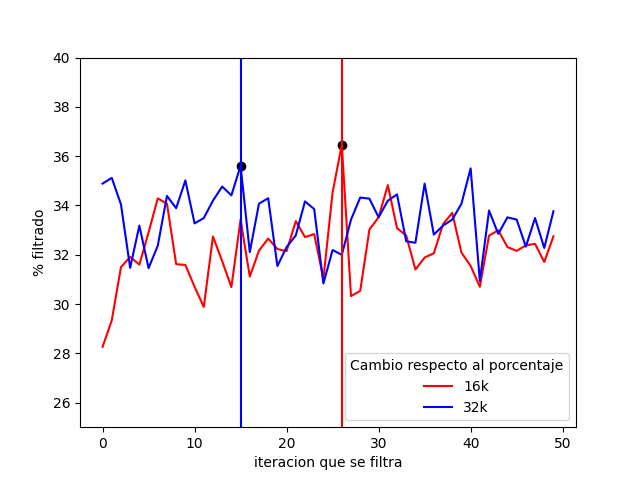
\includegraphics[scale=.7]{16_32.png}
  \caption{Gráfica de 16k y 32k de porcentaje filtrado por iteración.}
  \label{f1}
\end{figure}
\bigskip

En la figura \ref{f2} se obtiene el comportamiento para \texttt{64k y 128k}, se observa que el punto mas alto de porcentaje de cúmulos más grandes no tiene una relación de cambio con respecto a la figura \ref{f1} ya que los puntos dan al azar debido al comportamiento de partirse y aglomerarse de las partículas. 

\begin{figure}[H]
  \centering      
  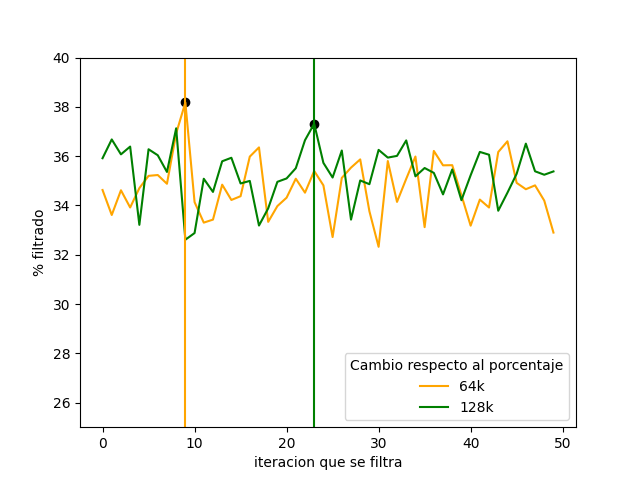
\includegraphics[scale=.7]{64_128.png}
  \caption{Gráfica de 64k y 128k de porcentaje filtrado por iteración.}
  \label{f2}
\end{figure}
\bigskip

\section{Conclusión}
En base a los resultados obtenidos se concluye que lo que se busca en ver como se comporta el porcentaje de partículas filtradas y ver su punto más alto no tiene una relación con respecto a la \texttt{n} que se varía debido a que los datos son muy aleatorios y generan diversos picos en la gráfica y los puntos altos están de igual manera aleatoriamente, lo que si tiene una cierta relación es que el porcentaje de las cuatro gráficas se mantuvo en rangos de entre veintiocho a treinta y ocho de porcentaje.

\bibliography{refe}
\bibliographystyle{plainnat}

\end{document}